\section{Results}

Our comparative analysis between \congruent and \incongruent interpolation paths reveals a dramatic divergence in geometric and semantic properties. \Tabref{tab:metrics} summarizes the key metrics, demonstrating the extreme non-linearity associated with \incongruent paths.

\begin{table}[h]
\centering
\caption{Comparison of geometric and semantic metrics between \congruent and \incongruent interpolation paths in \gpttwo (layer 6). \increase indicates a positive change from the start of the path toward the midpoint, and \decrease indicates a decrease.}
\label{tab:metrics}
\begin{tabular}{@{}lccc@{}}
\toprule
Metric & \related Path & \incongruent Path & Ratio / $\Delta$ \\
\midrule
Max Information Metric \infometric & 0.0084 & {\bf 4.0396} & {\bf $\approx$480$\times$} \\
Max \sae Reconstruction \mse & 0.4396 & {\bf 0.5747} & {\bf +30.7\%} \\
Mid-point Entropy Peak & -0.0061 & {\bf +0.1796} & {\bf Increased Uncertainty} \\
$\normlzero$ Sparsity Trend (mid - ends) & +2.5 & {\bf -27.0} & {\bf Sparsification} \\
\bottomrule
\end{tabular}
\end{table}

\para{Curvature and Information Speed.} The most striking finding is the 480$\times$ difference in the maximum information metric (\infometric). \Figref{fig:info_metric} shows the distribution of \infometric along the interpolation path. For \related concepts, such as ``Paris'' and ``Berlin,'' the transition in probability space is nearly flat, reflecting a smooth semantic blend. In contrast, the \incongruent path (e.g., ``Paris'' to ``fish'') shows a massive spike in \infometric at the midpoint. This indicates a ``cliff'' in the model's semantic manifold, where small movements in activation space cause catastrophic shifts in the output distribution.

\begin{figure}[h]
\centering
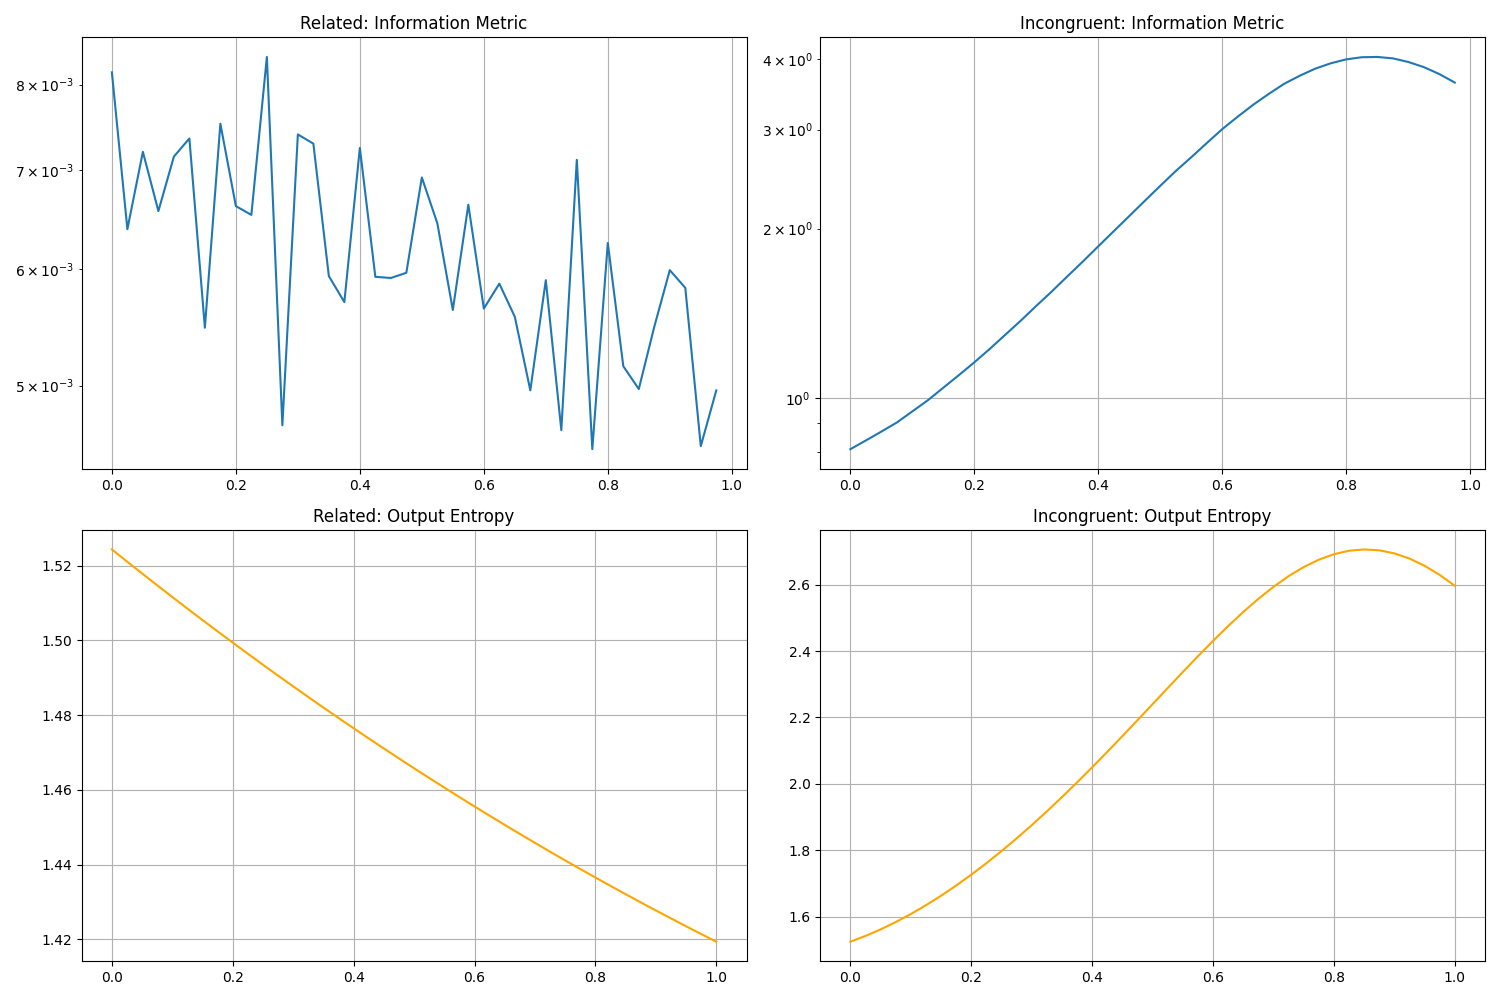
\includegraphics[width=0.7\linewidth]{figures/exp3_analysis.png}
\caption{Information metric \infometric along the interpolation path. \related paths (blue) remain flat, while \incongruent paths (red) show an extreme spike at the midpoint, indicating high local curvature.}
\label{fig:info_metric}
\end{figure}

\para{Manifold Drift and \sae Error.} The \sae reconstruction \mse provides a diagnostic for whether the linear path stays on the manifold of activation patterns seen during training. As shown in \Figref{fig:mse_hump}, \incongruent paths experience a 30.7\% increase in \mse compared to \related ones. This ``\mse hump'' suggests that \lerp between distant, unrelated concepts forces the model's hidden state into regions of ``no-man's land'' where the learned features are unable to accurately represent the vector.

\begin{figure}[h]
\centering
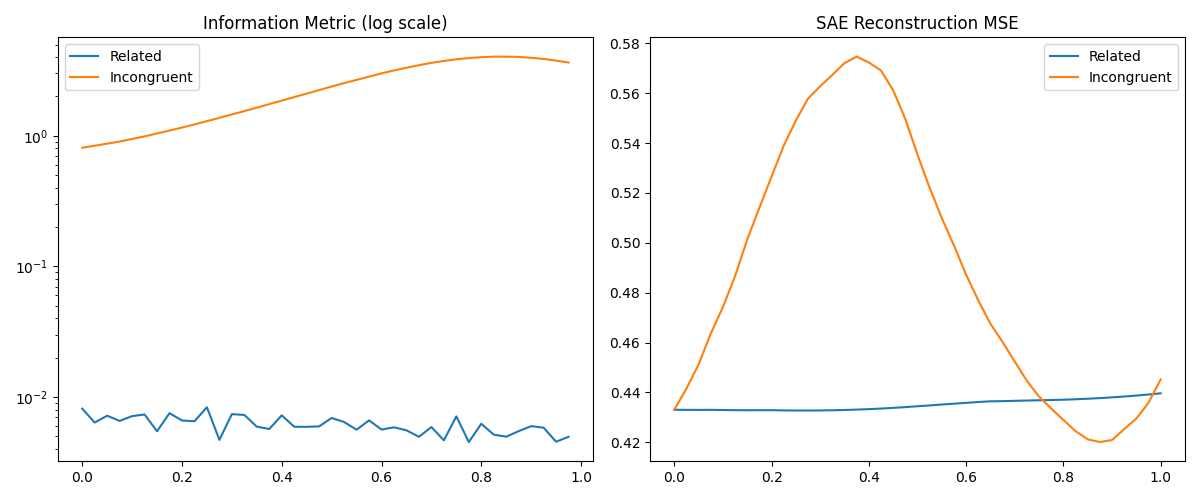
\includegraphics[width=0.7\linewidth]{figures/final_comparison.png}
\caption{Sparse Autoencoder (\sae) reconstruction Mean Squared Error (\mse) along the interpolation path. The \incongruent path exhibits a significant hump, indicating that the interpolated activations drift away from the model's learned feature manifold.}
\label{fig:mse_hump}
\end{figure}

\para{Output Uncertainty and Sparsification.} \Figref{fig:entropy_sparsity} illustrates the behavioral shift during \incongruent interpolation. While \related concepts often show a slight increase in $\normlzero$ sparsity (suggesting a superposition of features), \incongruent midpoints exhibit a massive decrease in $\normlzero$ ($-27.0$). This unexpected sparsification suggests that the model ``shuts down'' its specialized semantic features when forced into an incongruent state. Simultaneously, the output entropy peaks ($+0.1796$), indicating that the model's predictions become highly uncertain and confused as it drifts off-manifold.

\begin{figure}[h]
\centering
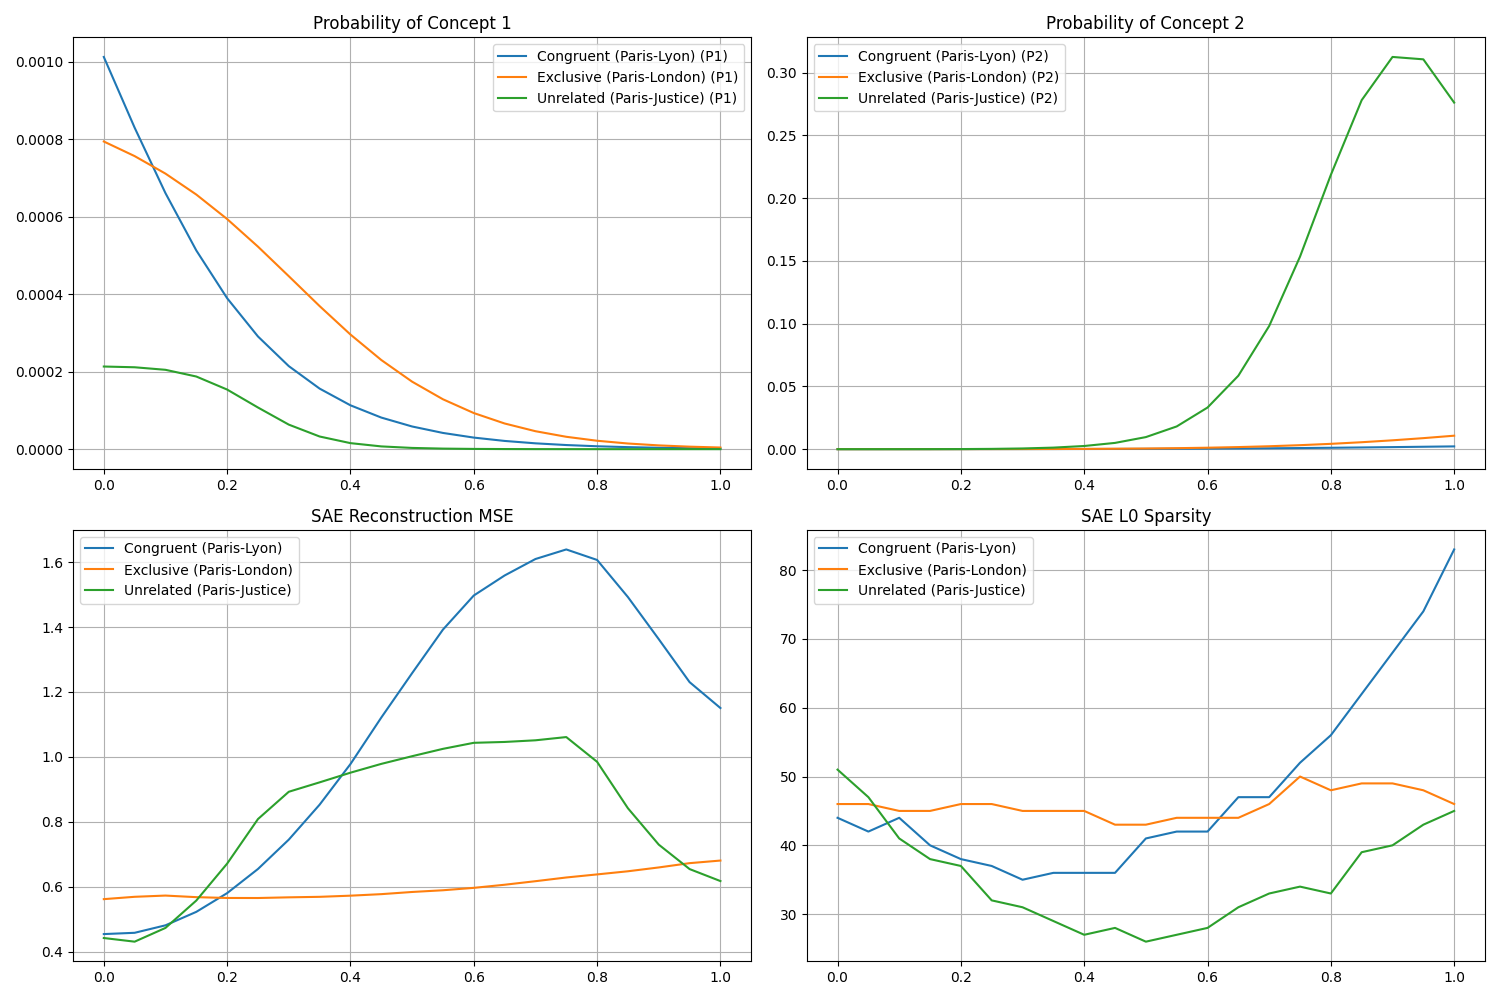
\includegraphics[width=0.7\linewidth]{figures/interpolation_analysis.png}
\caption{Analysis of output entropy and \sae $\normlzero$ sparsity along the path. The \incongruent path shows a peak in entropy and a dramatic dip in $\normlzero$, revealing a collapse of the model's semantic representations.}
\label{fig:entropy_sparsity}
\end{figure}

\para{Transition Dynamics.} For mutually exclusive concepts, we observed a ``Winner-Take-All'' transition, where the probability of the initial concept drops sharply while the second concept remains near zero, followed by a sudden jump. This bistability is a hallmark of the high curvature identified by our information metric.
